\documentclass[border=3pt]{standalone}
% Preâmbulo compartilhado pelos diagramas TikZ da aula 7 (Filtros Não Paramétricos)
\usepackage[T1]{fontenc}
\usepackage[utf8]{inputenc}
\usepackage{lmodern}
\usepackage{amsmath}
\usepackage{xcolor}
\usepackage{tikz}
\usetikzlibrary{arrows.meta,angles,quotes,decorations.pathmorphing,calc,
                positioning,shapes.geometric,shapes.misc,backgrounds,fit,
                math}

% Paleta (mesma dos SVGs originais)
\definecolor{dblue}{HTML}{2A5B8C}
\definecolor{dorange}{HTML}{B3541E}
\definecolor{dgreen}{HTML}{4A7C59}
\definecolor{dred}{HTML}{9C4B4B}
\definecolor{dcream}{HTML}{F4F1EA}
\definecolor{dshade}{HTML}{DDD7C9}

% Função gaussiana (não normalizada por padrão de escala visual)
\pgfmathdeclarefunction{gauss}{3}{%
  \pgfmathparse{1/(#3*sqrt(2*pi))*exp(-((#1-#2)^2)/(2*#3^2))}%
}

% Estilos comuns (prefixo d... para não colidir com chaves internas do pgf)
\tikzset{
  >={Stealth[length=2mm]},
  dguide/.style={gray!55, dashed, line width=0.4pt},
  daxis/.style={gray!60, line width=0.7pt, ->},
  dbody/.style={fill=black!3, draw=black!80, line width=1pt},
  dacc/.style={draw=dblue, line width=1pt},
  dlbl/.style={black!55, font=\small},
  dsub/.style={black!45, font=\footnotesize},
  dstate/.style={circle, draw=black!80, fill=dcream, line width=1pt,
                 minimum size=17mm, font=\large, inner sep=1pt},
  dobs/.style={circle, draw=black!80, fill=dshade, line width=1pt,
               minimum size=14mm, font=\large, inner sep=1pt},
  dbox/.style={rounded corners=2pt, draw=black!80, fill=dcream, line width=1pt,
               align=center, inner sep=6pt},
  dop/.style={circle, draw=black!80, fill=white, line width=1pt,
              minimum size=6mm, inner sep=0pt, font=\small},
  dtrans/.style={->, dblue, line width=1pt},
  dmeas/.style={->, dorange, line width=1pt},
  dcurve/.style={line width=1pt, dblue},
  dcurveb/.style={line width=1.4pt, dorange},
}

\begin{document}
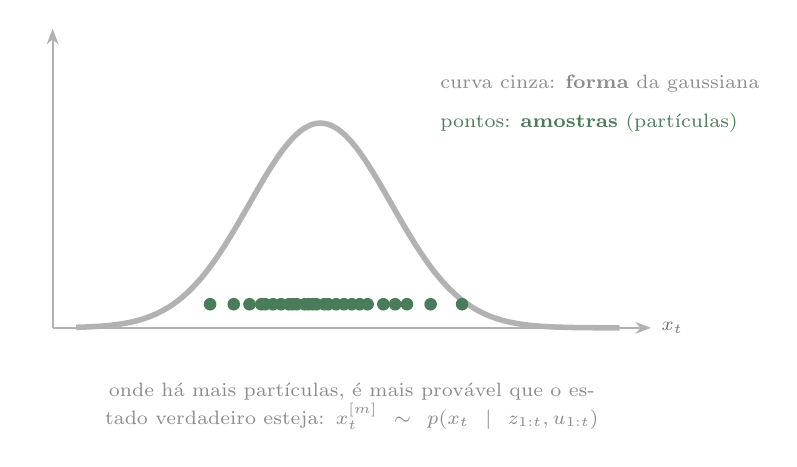
\begin{tikzpicture}[x=1cm,y=1cm]
  \draw[daxis] (0,0) -- (7.6,0) node[right, dlbl, font=\scriptsize] {$x_t$}; \draw[daxis] (0,0) -- (0,3.8);
  \draw[black!30, line width=2pt, domain=0.3:7.2, samples=80, smooth] plot (\x, {2.6*exp(-((\x-3.4)*(\x-3.4))/(2*0.9*0.9))});
  \foreach \x in {2.0,2.3,2.5,2.65,2.8,2.9,3.0,3.1,3.2,3.3,3.35,3.45,3.5,3.6,3.7,3.8,3.9,4.0,4.2,4.35,4.5,4.8,5.2,2.7,3.05,3.25} { \fill[dgreen] (\x,0.3) circle (0.08); }
  \node[dsub, font=\scriptsize, anchor=west] at (4.8,3.1) {curva cinza: \textbf{forma} da gaussiana};
  \node[dgreen, font=\scriptsize, anchor=west] at (4.8,2.6) {pontos: \textbf{amostras} (partículas)};
  \node[dsub, font=\scriptsize, align=center, text width=8cm] at (3.8,-1.0) {onde há mais partículas, é mais provável que o estado verdadeiro esteja: $x_t^{[m]}\sim p(x_t\mid z_{1:t},u_{1:t})$};
\end{tikzpicture}
\end{document}
